\Chapter{MAGNIS (MAGnetized Negative Ion Source)}
\begin{refsection}

\chaptermark{Modèles plasmas froids magnétisés}

Dans ce chapitre, nous proposons un nouveau modèle fluide pour décrire le
transport magnétisé dans les plasmas froids. Nous discutons tout d'abord de
l'approche standard de modélisation des plasmas froids, des problématiques qui
lui sont propres ainsi que des difficultés rencontrées lors du développement du
modèle basé sur les vitesses de dérive. La suite concerne l'élaboration du
nouveau modèle, nous le dérivons en expliquant les différents termes essentiels
à description du transport dans les plasmas froids puis nous détaillons le
schéma numérique original utilisé pour résoudre les équations.
Une dernière partie est consacrée à la vérification du code par une étude de
convergence sur maillage et à une validatation élémentaire du comportement du
plasma dans des cas théoriques représentatifs.

\section{Problématique}

La compréhension de l'origine et de la nature du transport dans les plasmas
magnétisés est un enjeu majeur pour la conception, la réalisation et
l'optimisation de nombreuses applications et procédés. Dans les sources plasmas
fonctionnant à basse pression,  La plupart des modèles fluides décrivant les
phénomènes de transport magnétisés dans les plasmas froids sont basés sur les équations de dérive-diffusion (\S \ref{1-deriveDiffMag}). Cependant, au delà d'une certaine intensité de champ magnétique, l'anisotropie du transport rend la résolution numérique de ces
équations complexe voire impossible\footnote{Le problème est alors généralement
adressé à travers le développement de modèles cinétiques numériquement très
coûteux, et nécessitant à priori la résolution d'échelles de l'ordre de la
longueur de Debye et de la fréquence plasma.}.
Celles-ci sont en fait peu adaptées au transport fortement
magnétisé~\cite{Golant}.


Un indice nous est donné en considérant la description du transport transverse
par les vitesses de dérive (cf.
introduction) où l'équilibre des courants fait intervenir la divergence de la
dérive de polarisation. Cette dérive, essentielle dans la dynamique du transport
transverse, est absente du modèle qui néglige totalement l'inertie des
particules. Le modèle de dérive-diffusion cherche une solution stationnaire à un
problème intrinsèquement non-stationnaire.
\parencite{Fruchtman}
\parencite{Sternberg}
D'un autre côté,

\section{Description du modèle}
Le plasma est constitué d'électrons et d'une ou plusieurs espèces d'ions de
charge $q_\alpha$ et de masse $m_\alpha$. On considère un plasma de taille $L$,
confiné et en interaction avec des parois à travers une gaine large de quelques longueurs
de Debye. La longueur $L$ est prise suffisement grande $L\gg\lambda_D$ pour
supposer le plasma quasi-neutre. Le champ magnétique $\mathbf{B}$ imposé est 
stationnaire, de sorte que le champ électrique dérive directement d'un 
potentiel électrostatique $\mathbf{E}=-\nabla U$. Le transport est décrit
dans le plan perpendiculaire au champ magnétique et tient compte des pertes à
la paroi dans la direction parallèle en les intégrant le long des lignes de champ.

\subsection{Equations de conservation}
Pour décrire l'évolution des espèces dans un plasma partiellement ionisé, basse
pression et magnétisé, l'équation du mouvement doit tenir compte de
l'interaction avec le gaz, de l'inertie et du terme de Laplace :

\begin{equation}
\partial_t \mathbf{u}_\alpha + \mathbf{u}_\alpha\cdot\nabla\mathbf{u}_\alpha+
\nu_\alpha\mathbf{u}_\alpha+\omega_{c\alpha}\mathbf{b}\times\mathbf{u}_\alpha=
-\frac{q_\alpha}{m_\alpha}\left(\nabla U+\frac{\nabla
p_\alpha}{q_\alpha n_\alpha}\right)
\end{equation}

où $n_\alpha$ est la densité de l'espèce considérée, $\mathbf{u}_\alpha$ sa
vitesse fluide, $p_\alpha$ la pression (dont nous ne retenons que la
contribution isotrope) et $U$ le potentiel électrostatique. La fréquence
cyclotronique est notée $\omega_{c\alpha}=q_\alpha B/m_\alpha$ et $\nu_\alpha$
est une fréquence effective rendant compte des collisions.
Le transfert de quantité de mouvement dû aux collisions contient la perte liée à
l'ionization
$\nu_\alpha=\nu_{\alpha}^{iz}+\nu_{\alpha}^{c}+\nu_{\alpha}^{ei}$ où
$\nu_{\alpha}^{c}$ et $\nu_{\alpha}^{ei}$ sont respectivement les
fréquences de collisions particules chargées - neutres et de collisions
coulombiennes.

L'évolution de chaque espèce est décrite par une équation de continuité :

\begin{equation}
\label{3-continuite}
\partial_t n_\alpha +
\nabla\cdot\left(n_\alpha\mathbf{u}_\alpha\right)=S_\alpha(T_e)
\end{equation}

avec $S_\alpha$ un terme d'ionisation, fortement dépendant de la
température électronique $T_e$. En considérant l'hypothèse de quasi-neutralité, la somme des
équations de continuité conduit à l'équation de conservation du courant :

\begin{equation}
\label{eqCourant}
\nabla\cdot(\sum_ien_i\mathbf{u}_i-en_e\mathbf{u}_e)=0
\end{equation}

où l'indice i dénote éventuellement différentes espèces d'ions. 
L'équation \eqref{eqCourant} couple les différentes espèces en contrôlant
l'évolution du potentiel électrostatique $U$.

L'équation de conservation de l'énergie est obtenue classiquement en substituant
l'équation de continuité afin d'éliminer le terme convectif :

\begin{equation}\begin{split}
\label{3-energie}
\frac{3}{2}en_e\partial_tT_e + \nabla\cdot(\mathbf{q_e}) +
(\frac{5}{2}S_e-\partial_tn_e)eT_e \\=n_e\mathbf{u}_e\cdot(\nabla
U-\frac{5}{2}e\nabla T_e)+n_e\left(P_{ext}-\Pi\right)
\end{split}
\end{equation}

où $T_e$ est la température électronique exprimée en eV, $S_e$ est le
terme source d'électrons lié à l'ionisation, $P_\text{ext}$ la puissance
extérieure déposée dans le plasma et $\Pi$ le terme de perte d'énergie dûe aux
collisions. La fermeture du modèle se fait alors sur le flux de chaleur
$\mathbf{q}_e$, tel qu'exprimé par
V.E. Golant dans~\cite{Golant} :

\begin{equation}
\partial_t \mathbf{q}_e + \nu_e\mathbf{q}_e+\omega_e\mathbf{q}_e\times\mathbf{b} =
-\frac{5}{2}\frac{e^2}{m_e}n_eT_e\nabla T_e
\end{equation}

Le flux de chaleur est magnétisé de la même façon que le flux de matière et
dépend essentiellement du gradient de température. Dans les sources magnétisées,
où la longueur de gradient thermique est de l'ordre de la largueur
du filtre magnétique, le flux de chaleur influence fortement le transport
transverse. Il doit donc nécessairement être pris en compte et décrit
avec le minimum d'approximations.

\subsection{Conditions aux limites}
Le modèle quasineutre est complété par la
définition des conditions aux limites portant sur les flux et intégrant le
maximum de considérations physiques. Dans le cas d'une paroi conductrice, un
modèle classique de gaine non-collisionnelle est utilisé. Les flux ioniques et
le flux électronique sont définis en l'entrée de gaine par :

\begin{align}
&\Gamma_i=n_i\mathbf{u}_i\cdot\mathbf{n}=n_i.\max\left(c_s,\mathbf{u_i}\cdot\mathbf{n}\right)
\\
&\Gamma_e=n_e\mathbf{u}_e\cdot\mathbf{n}=n_e\frac{1}{2\sqrt{\pi}}v_{Te}=n_ec_s\exp(\Lambda-\Delta
U/T_e)
\end{align}

avec $\mathbf{n}$ le vecteur normal à la paroi,
et $c_s=(eT_e/m_i)^{\text{\textonehalf}}$ la vitesse acoustique ionique. Le flux
d'électron est obtenu en considérant une fonction de distribution maxwellienne, 
que l'on intègre sur le demi-espace des vitesses dirigées vers la paroi avec 
$v_{Te}=(2eT_e/m_e)^{\text{\textonehalf}}$ la vitesse électronique thermique.
La différence entre le potentiel plasma $U$ et le potentiel de la paroi
$U_w$ se réécrit pour un courant nul:

\begin{equation}
	\mathbf{j}\cdot\mathbf{n}=0\Leftrightarrow \Delta U=U-U_w =
T_e(\Lambda-ln\sum_i\mathbf u_i/c_s)
\end{equation} 

où le potentiel flottant $\Lambda$ est défini pour un plasma
n'étant composé que d'une espèce :

\begin{equation}
	\Lambda=ln\left(\frac{eT_e}{2\pi
	m_e\mathbf{u}_i^2}\right)^{\text{\textonehalf}} \le 
	ln\left(\frac{m_i}{2\pi m_e}\right)^{\text{\textonehalf}}
\end{equation}

Les ions sont perdus au minimum avec la vitesse acoustique, mais
éventuellement avec une vitesse supersonique. Le flux d'électron s'ajuste
quant à lui pour réguler la valeur du potentiel flottant autour de La condition
limite pour le courant est par conséquence définie par :

\begin{equation}
\mathbf{j}\cdot\mathbf{n}=e\sum_in_i{\mathbf u}_i-en_ec_s\exp(\Lambda-\Delta
U/T_e)
\end{equation}

Si la paroi est isolante, la surface se polarise pour assurer la nullité du
courant sortant :

\begin{equation}\begin{split}
\mathbf j\cdot\mathbf{n}=0\Leftrightarrow
U_w=U-T_e(\Lambda-ln\sum_i\mathbf u_i/c_s)
\end{split}\end{equation}

L'énergie perdue par les électrons en entrée de gaine s'obtient en
additionnant l'énergie moyenne perdue à la paroi (intégrée sur une distribution
semi-maxwellienne) et l'énergie transférée aux ions dans la chute de potentiel :

\begin{equation}
	\varepsilon_w=2T_e+\Delta U
\end{equation}
 
 On peut alors relier cette perte totale aux flux sortants de l'équation
 d'énergie \eqrefp{3-energie}, qui correspondent au flux d'énergie porté par
 les particules et au flux de chaleur :
 
\begin{equation}
\Gamma_\varepsilon=\frac{5}{2}{\Gamma}_eT_e+\mathbf{q}_e\cdot\mathbf{n}=
\Gamma_e\left(2T_e+\Delta U\right)
\end{equation}

En regroupant les termes portant sur le flux d'électron, on peut exprimer la
condition limite pour le flux de chaleur :

\begin{equation}
\mathbf{q}_e\cdot\mathbf{n}=\Gamma_e\left(\Delta U-\frac{1}{2}T_e\right)
\end{equation}

Ces conditions aux limites sont justifiées dans des plasmas non-magnétisés et à
l'extrémité de lignes de champ interceptant la paroi dans
des plasmas magnétisés. Dans la direction perpendiculaire au champ magnétique,
nous gardons comme hypothèse que le la vitesse ionique doit au
minimum atteindre la vitesse de Bohm pour permettre une brisure de
la quasineutralité du plasma et l'apparition d'une gaine de charge d'espace
positive.

\subsection{Réduction 2D du modèle}
Le système d'équations Eqs.(\ref{3-continuite}~-~\ref{3-energie}) décrit le
transport magnétisé dans un plasma froid en suivant l'évolution des densités de
particules $n_\alpha$, du potentiel électrique $U$ et de la température
électronique $T_e$ dans un espace à trois dimensions.

Le long des lignes de champ, les électrons sont collisionnels et en équilibre de
Boltzmann, entraînant une rapide homogénéisation des quantités macroscopiques
du plasma dans la direction du champ magnétique. 
En considérant une moyenne effective le long des lignes de
champ, le système est intégré dans la direction parallèle et peut se réécrire :

\begin{align}
\label{3-equations2D}
\partial_t {n}_\alpha& +
\nabla_\perp\cdot\left({n}_\alpha\mathbf{u}_{\alpha\perp}\right)=S_\alpha({T}_e)
- \Gamma_{\alpha\para}\\[0.5cm]
\nabla_\perp\cdot&(\sum_ie{n}_i\mathbf{u}_{i\perp}
-e{n}_e\mathbf{u}_{e\perp})= - \nabla_\para j_\para\\[0.5cm]
\begin{split}\frac{3}{2}{n}_e&\partial_t{T}_e +
\nabla_\perp\cdot(\mathbf{q}_{e\perp}) +
(\frac{5}{2}S_e-\partial_t\tilde{n}_e)\tilde{T}_e =\\
&\tilde{n}_e\mathbf{u}_{e_\perp}\cdot(\nabla_\perp
\tilde{\Phi}-\frac{5}{2}\nabla_\perp
\tilde{T}_e)+\tilde{n}_e\left(P_{ext}-\Pi\right)-\Gamma_{\varepsilon\para}
\end{split}
\end{align}

où les grandeurs sont des moyennes effectives le long de la direction parallèle $\tilde{x}=<x>_\para$ 
et où le mouvement parallèle se réduit aux pertes de particules $\Gamma_n$, de
courant $\Gamma_\rho$ et d'énergie $\Gamma_\varepsilon$ au bout des lignes de
champ. Dans la suite, nous laissons de côté la notation de moyenne, l'indice
perpendiculaire et nous ne considérons qu'une espèce d'ion afin de simplifier
les notations.

\section{Implémentation numérique}

MAGNIS résout le système d'équations \ref{3-equations2D} de manière implicite
les termes influençants non-négligemment le transport magnétisé dans les
plasmas froids. Le domaine de simulation est le plan perpendiculaire à
$\mathbf{b}$, rectangulaire et maillé uniformément suivant les directions
$\mathbf{x}$ et $\mathbf{y}$. Les quantités scalaires sont définies aux noeuds
du maillage et les composantes vectorielles entre les points de maillage.

 \subsection{Discrétisation spatiale}
\begin{figure}[htbp]
\centering
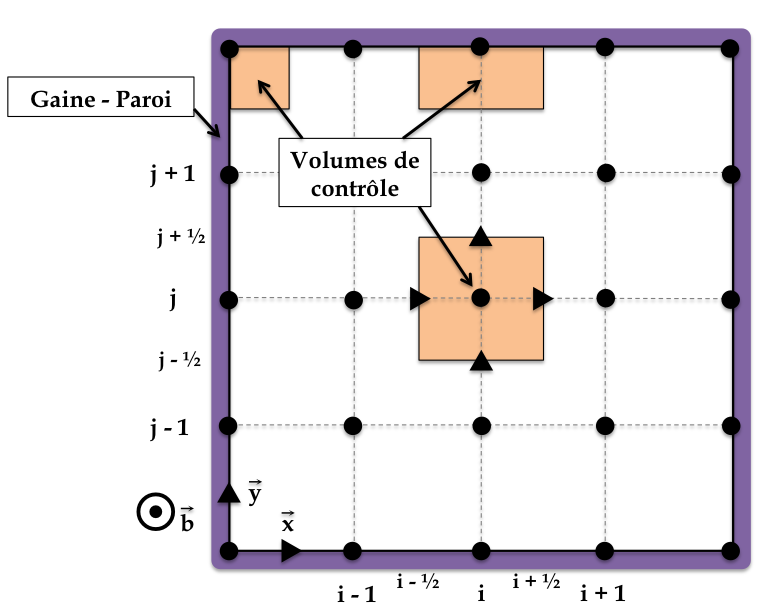
\includegraphics[height=64mm,width=80mm]{figures/3-magnisGrid.png}
{\caption{Maillage 2D pour les schémas volumes finis}
\label{maillage}}
\end{figure}

 \subsection{Fréquences}
 \parencite{Phelps}
 Une attention particulière est portée à description précise des 
 flux de matière et de chaleur fortement dépendants de la magnétisation du
 plasma. Une étape de prédiction est tenant compte de la force


\subsection{Discrétisation temporelle}

\begin{equation}
S_s(T_e)=n^{k+1}n_gk_{s}^{iz}(T_e)
\end{equation}
où $n_g$ est la densité du gaz et $k_{s}^{iz}$ le coefficient d'ionisation spécifique à l'espèce.
\cite{Hemsworth}

\section{Vérification et validation}

\subsection{Etude de convergence en temps et en espace}
\subsubsection{Densité}
\subsubsection{Potentiel}
\subsubsection{Température}
\subsection{Influence du champ magnétique}
\subsection{Réponses à la température}

%\bibliographystyle{alpha}
%\bibliography{biblio}
\end{refsection}

